% tbsrc/projection.tex — The Forward Model: Projection
% Status: written (first draft). Physics content migrated from the retired
% docs/tex/joseph3d_note.tex; port/implementation details live in the
% RecoCrysp Documenter pages, not here.
\section{The Forward Model: Projection}
\label{sec:projection}

The forward projector is the operator that turns an activity image into the
mean data the scanner would record. Section~\ref{sec:intro:problem} introduced
it abstractly as the system matrix $\Aop$ in $\pred = \Aop\,\xv$; this section
makes it concrete --- what $\Aop$ computes, how \code{RecoCrysp} evaluates it
with Joseph's method, and why its transpose $\Aadj$ must be the \emph{exact}
adjoint.

\subsection{The line integral and the system matrix}
\label{sec:projection:lineintegral}

Let $f(\bm{u})$ be the continuous activity field of
Section~\ref{sec:intro:problem}. In the idealized non-TOF model the expected
number of true coincidences on LOR $i$, with endpoints
$\bm{x}_s^{(i)}$ and $\bm{x}_e^{(i)}$
(Section~\ref{sec:geometry}), is the integral of $f$ along the line,
\begin{equation}
  p_i \;=\; \int_{\mathrm{LOR}_i} f(\bm{u})\,\mathrm{d}\ell .
  \label{eq:proj-lineintegral}
\end{equation}
The image is stored on a voxel grid (Section~\ref{sec:grid}) as the vector
$\xv\in\RR^N_{\ge0}$, and $f$ is reconstructed between grid points by
\emph{trilinear interpolation}; write $\tilde f$ for this interpolated field, so
that $\tilde f$ is linear in the voxel values $\xv$. Equation
\eqref{eq:proj-lineintegral} evaluated on $\tilde f$ is therefore linear in
$\xv$, and collecting all LORs gives the matrix form
\begin{equation}
  \pred \;=\; \Aop\,\xv ,
  \qquad
  \Aop \in \RR^{M\times N},
  \label{eq:proj-matrix}
\end{equation}
already met as \eqref{eq:intro-ideal}. Row $i$ of $\Aop$ holds the contribution
of each voxel to LOR $i$; it has only a handful of nonzeros (the voxels the ray
actually crosses), so $\Aop$ is extremely sparse. Crucially it is never formed:
\code{RecoCrysp} applies $\Aop$ and $\Aadj$ \emph{matrix-free}, recomputing the
weights on the fly for each LOR, which is what makes millions of LORs and
millions of voxels tractable.

\subsection{Joseph's method}
\label{sec:projection:joseph}

A direct evaluation of \eqref{eq:proj-lineintegral} would resample $\tilde f$ at
many points along each ray. Joseph's method~\cite{joseph1982} is a more
efficient and accurate quadrature that steps through the image one voxel plane
at a time. It first selects the \emph{principal axis} $d$ of the ray --- the
coordinate axis along which the ray travels fastest, i.e.\ the one with the
largest squared direction cosine,
\begin{equation}
  d \;=\; \argmax_{k\in\{1,2,3\}} \cos^2\theta_k ,
  \qquad
  \cos\theta_k \;=\; \frac{\Delta r_k}{\norm{\Delta\bm{r}}} ,
  \qquad
  \Delta\bm{r} \;=\; \bm{x}_e - \bm{x}_s .
  \label{eq:proj-principal}
\end{equation}
The integral is then approximated as a sum over the voxel planes perpendicular
to $d$,
\begin{equation}
  p_i \;\approx\; c \sum_{j=j_{\min}}^{j_{\max}}
      \mathcal{B}_d[\tilde f]\!\left(\bm{u}_j\right) ,
  \qquad
  c \;=\; \frac{\Delta_d}{\abs{\cos\theta_d}} ,
  \label{eq:proj-joseph}
\end{equation}
where $\mathcal{B}_d[\tilde f](\bm{u}_j)$ is the \emph{bilinear} interpolation
of the image within plane $j$, evaluated at the point $\bm{u}_j$ where the ray
pierces that plane, and $\Delta_d$ is the voxel size along $d$. Stepping along
the fastest axis guarantees that the ray crosses exactly one plane per voxel
step, so no plane is skipped or double-counted. Each plane contributes the
interpolated value sampled \emph{within} the plane (a $2\times2$ weighting),
while the geometric spacing between samples along the ray is folded into the
single \emph{path-length correction factor} $c$: the planes are a distance
$\Delta_d$ apart along $d$, but the ray segment between them is longer by
$1/\abs{\cos\theta_d}$, and $c$ converts the plane-by-plane sum back into a
length-weighted integral. Figure~\ref{fig:joseph} shows the construction.

\begin{figure}[t]
  \centering
  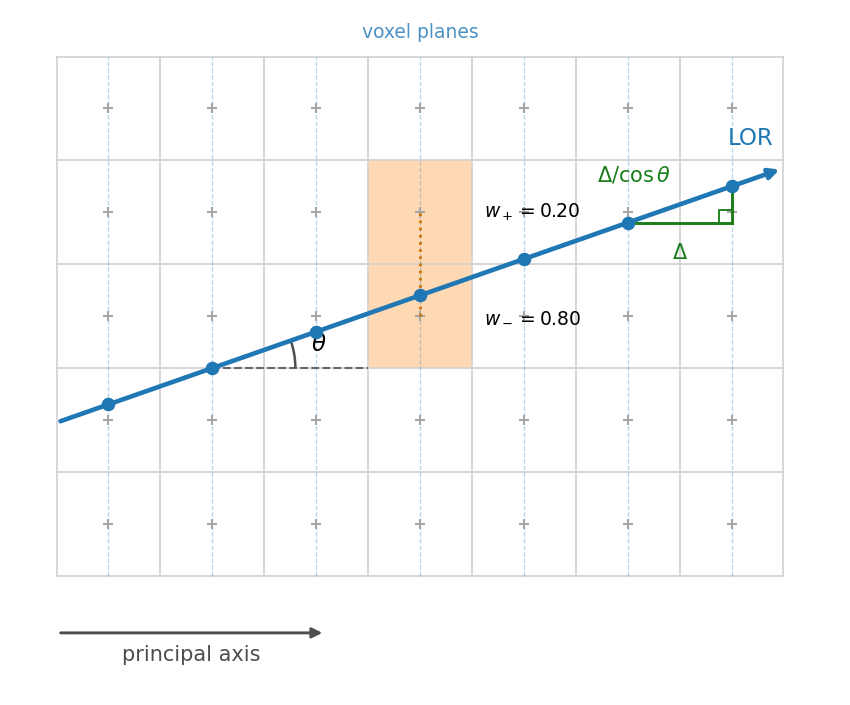
\includegraphics[width=0.82\textwidth]{figures/joseph_principle.png}
  \caption{Joseph's method (2D schematic). The ray's principal axis is
    horizontal; the method steps over the voxel planes perpendicular to it
    (dashed) and, at each crossing (dots), interpolates the image between the
    bracketing voxels with weights $w_\pm$ that sum to one (shaded column). The
    plane sum is then scaled by the correction factor $\Delta/\cos\theta$, the
    ratio of the ray segment between planes to their spacing $\Delta$. In 3D the
    in-plane interpolation is bilinear, over the four surrounding voxels.}
  \label{fig:joseph}
\end{figure}

Two properties make this cheap. The crossing points $\bm{u}_j$ advance by a
\emph{constant} increment from plane to plane, so the inner loop reduces to two
additions and one bilinear interpolation (four image samples) per plane. And
the traversal limits $j_{\min},j_{\max}$ follow from intersecting the ray with
the image bounding box, so only voxels actually on the ray are touched; rays
that miss the volume contribute zero.

\begin{remark}
The endpoints in \eqref{eq:proj-principal} are arbitrary world-space points, not
detector-element centres. The projector is therefore \emph{endpoint-driven}: it
integrates a thin line between whatever two points it is given and knows nothing
about crystal size or detector technology (Section~\ref{sec:geometry}). Finite
detector resolution is a separate operator $\Gop$, applied to the image before
projection (Section~\ref{sec:resolution}); it is deliberately not part of
$\Aop$.
\end{remark}

\subsection{Back-projection and the matched adjoint}
\label{sec:projection:adjoint}

Iterative reconstruction (Sections~\ref{sec:mlem}--\ref{sec:acceleration})
needs not only $\Aop$ but its transpose $\Aadj$, the \emph{back projector}.
Where the forward projector \emph{gathers} a value for each LOR from the voxels
it crosses, the back projector \emph{scatters} a per-LOR quantity $y_i$ back
into those same voxels:
\begin{equation}
  \bigl(\Aadj\,\yv\bigr)_v \;=\; \sum_i A_{iv}\,y_i .
  \label{eq:proj-back}
\end{equation}
\code{RecoCrysp} computes \eqref{eq:proj-back} by walking each ray exactly as in
the forward pass and adding $c\,y_i$ into the four bilinear voxels of every
plane, with the \emph{same} weights $A_{iv}$ used in the forward direction.
Because many LORs write to the same voxel, these updates are accumulated
atomically.

Using the identical weights in both directions is what makes the pair
\emph{matched}: $\Aadj$ is the true transpose of $\Aop$, so for any image $\xv$
and any data $\yv$,
\begin{equation}
  \inner{\Aop\,\xv}{\yv} \;=\; \inner{\xv}{\Aadj\,\yv} .
  \label{eq:proj-adjoint}
\end{equation}
This is not a cosmetic nicety. The convergence guarantees of MLEM and OSEM ---
that each iteration does not decrease the likelihood --- rest on $\Aadj$ being
the exact adjoint of the $\Aop$ used in the same update
(Section~\ref{sec:mlem}). An \emph{unmatched} projector/back-projector pair
(for instance a forward Joseph projector with a structurally different,
faster back projector) breaks \eqref{eq:proj-adjoint} and can stall or bias the
reconstruction. \code{RecoCrysp} therefore derives both directions from one
kernel and verifies \eqref{eq:proj-adjoint} numerically.

\subsection{Precision and validation}
\label{sec:projection:validation}

All projector arithmetic is single precision (\code{Float32}), matching the
reference implementation \code{parallelproj}~\cite{schramm2024} and the
requirements of the GPU backends (Section~\ref{sec:intro:scope}). Two checks pin
down correctness on every backend:
\begin{itemize}
  \item \textbf{Analytic line integrals.} An axis-aligned ray through a uniform
        image of $n$ unit voxels of size $\Delta$ must integrate to exactly
        $n\Delta$; \code{RecoCrysp} reproduces this to \code{Float32} machine
        precision.
  \item \textbf{Adjointness.} For random images and random LORs, the two sides
        of \eqref{eq:proj-adjoint} (accumulated in double precision for the
        comparison) agree to a relative deviation of order $10^{-10}$,
        confirming the back projector is the exact transpose.
\end{itemize}

In code, the two operators are a single call each: the LOR endpoints are passed
as $3\times M$ matrices and the grid as its origin and voxel size.
\begin{lstlisting}
proj  = joseph3d_fwd(xstart, xend, img, img_origin, voxsize)   # p = A x
bimg  = joseph3d_back(xstart, xend, proj, size(img), img_origin, voxsize) # A' y
\end{lstlisting}
The same source runs on multithreaded CPUs and on GPUs (including Apple Metal)
unchanged; the backend follows the array type of the arguments. These are the
building blocks every later section composes into a full reconstruction.
